%%
%% Zhe Zhang - English Resume
%%

\documentclass{resume}

\setmainfont{Times New Roman}
\setmonofont{Menlo}

% Keep the English version compact enough for a two-page resume.
\usepackage{enumitem}
\setlist[itemize]{itemsep=1pt, topsep=2pt, parsep=0pt, partopsep=0pt}
\setlist[itemize,2]{itemsep=1pt, topsep=1pt, parsep=0pt, partopsep=0pt}
\setlength{\emergencystretch}{1em}

\fileinfo{%
  \faCopyright{} 2026, Zhe Zhang \hspace{0.5em}
  \faEdit{} \today
}

\name{Zhe}{Zhang}
\makeatletter
\def\@photo@width{2.00cm}
\def\@photo@position{right}
\def\@photo{%
  \begin{minipage}{\@photo@width}
    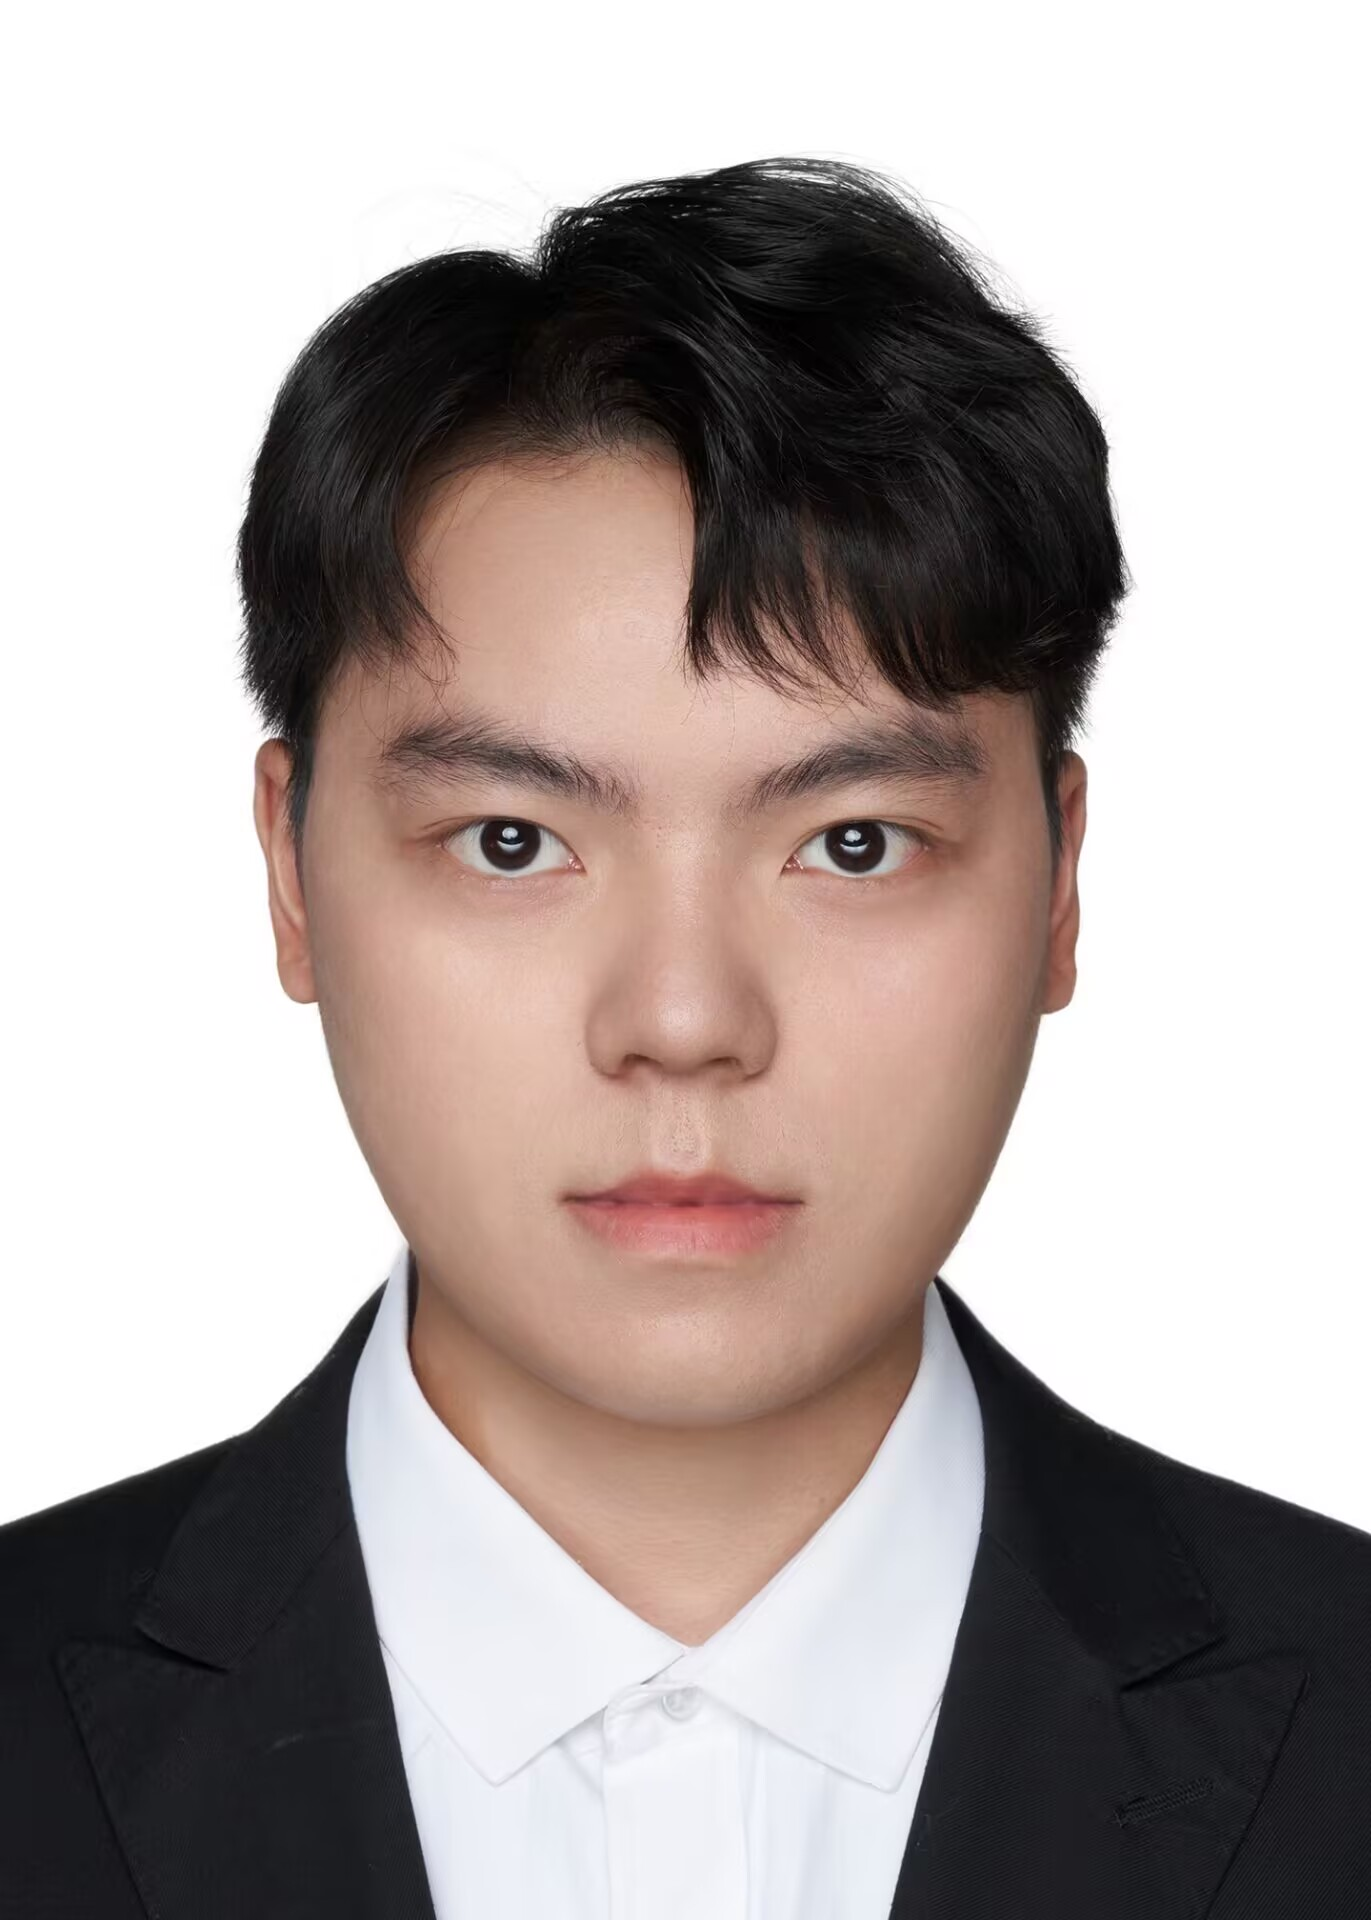
\includegraphics[width=\linewidth]{zhangzhe.jpg}%
  \end{minipage}%
}
\makeatother
\tagline{LLM Agent Engineer | AI Application Engineer}
\keywords{LLM Agents, Agent Runtime, RAG, MCP, Tool Use, Multimodal Memory, Python, TypeScript}

\profile{
  \mobile{13160006317}
  \email{3220857484@qq.com}
  \university{NJUST}\\
  \degree{M.S. in Software Engineering, in progress}
}

\begin{document}
\makeheader

\begin{abstract}
M.S. candidate in Software Engineering focused on LLM agents and AI application engineering. Contributing to the JF-AIX enterprise agent platform by building runtime control loops, multimodal file memory, cross-session long-term memory, observability, and product data loops. Leading an educational-content question authoring and review system that connects PDF parsing, OCR, quality control, and data ingestion. Previous experience includes semantic retrieval, recommendation, and monitoring for an aerospace AI model management platform.
\end{abstract}

\sectionTitle{Education}{\faGraduationCap}
\begin{itemize}
  \item \textbf{Nanjing University of Science and Technology} \textbullet{} M.S. in Software Engineering \hfill 2024.09 - Present
  \item \textbf{Nantong University} \textbullet{} B.S. in Software Engineering \hfill 2019.09 - 2023.06
\end{itemize}

\sectionTitle{Experience}{\faBriefcase}
\begin{itemize}
  \item \textbf{CETC 28th Research Institute} \hfill 2025.09 - 2026.04
  \begin{itemize}
    \item Contributed to an aerospace AI model lifecycle platform covering models, algorithms, datasets, container images, and deployment monitoring.
    \item Built semantic retrieval with Qwen3-Embedding-0.6B and FAISS by composing model names, categories, descriptions, linked datasets, and version notes into searchable documents for natural-language model discovery.
    \item Implemented model-resource recommendation by combining user history, resource-type preferences, and recent popularity; added user-scoped Redis caching for frequent recommendations to reduce duplicate computation and API jitter.
    \item Added operational monitoring and analysis with psutil, DBSCAN anomaly detection, and linear-regression forecasts of seven-day resource trends to surface capacity risks earlier.
  \end{itemize}

  \item \textbf{JF-AIX | Enterprise Agent Digital Workforce Platform} \hfill 2026.05 - 2026.08
  \begin{itemize}
    \item \textbf{Agent Runtime and edge-cloud coordination:} Contributed to an Electron + Vue 3 execution layer and NestJS control plane; took over a custom Agent Loop through the Pi Agent SDK and connected model inference, Tool/Skill execution, human approval, and persistence with circuit breaking, argument validation, output truncation and continuation, abort handling, and streaming events.
    \item \textbf{Session-level multimodal file memory:} Designed a first-turn raw-content injection -> asynchronous summarization and image description -> summary reference -> on-demand precise readback flow for small documents, images, and spreadsheets. Used renderer state, Electron local cache, and server metadata as three storage layers, with context-budget allocation, \texttt{documentId + hash} validation, atomic writes, and Draft Session migration for restart recovery and consistency.
    \item \textbf{Cross-session long-term memory:} Designed an isolated user-memory pipeline that asynchronously extracts stable \texttt{user}, \texttt{feedback}, \texttt{project}, and \texttt{reference} facts after each turn, persists them in MySQL, retrieves candidates through Elasticsearch vector search, and uses an LLM to select task-relevant memories before injecting L6 dynamic context scoped by user and Agent.
    \item \textbf{Observability and product data loop:} Established 12 standard event types across core domains. Implemented a locally persisted Desktop queue with 30-second batch flushing, 100 events per batch, a 2,000-event retention cap, and offline retry; derived server-side events asynchronously with \texttt{dedupHash} idempotency while excluding message bodies and file contents from telemetry.
  \end{itemize}
\end{itemize}

\newpage
\sectionTitle{Selected Project}{\faCode}
\begin{itemize}
  \item \textbf{Educational Content Question Authoring and Review System} \hfill 2026.02 - Present
  \begin{itemize}
    \item Built a Vue 3 + TypeScript workbench and Fastify + Prisma + PostgreSQL + Redis backend to replace spreadsheet and multi-tool workflows, covering textbook upload, PDF viewing, region-based OCR, human correction, quality control, and ingestion.
    \item Developed automated question segmentation using MinerU block coordinates and table-of-contents structure, followed by LLM extraction of question numbers, stems, options, answers, and explanations. Matched questions and answer keys by chapter title + question number when source pages were separated.
    \item Offloaded PDF splitting, MinerU parsing, OCR, and question segmentation to BullMQ workers; returned job IDs from APIs and streamed progress through SSE instead of blocking HTTP requests for minute-scale jobs.
    \item Built an ops-monitor service with Prometheus + Grafana for API latency, queue backlog, task wait and execution P95, and worker heartbeat metrics; configured alerts for offline workers, API P95 breaches, and high machine CPU.
  \end{itemize}
\end{itemize}

\sectionTitle{Awards}{\faTrophy}
\begin{itemize}
  \item \textbf{ICCV 2025 Perception Test Challenge - Multimodal Video Understanding and Visual Reasoning} \hfill Champion
  \begin{itemize}
    \item Fine-tuned Qwen2.5-VL-7B for multiple-choice video QA and addressed fine-grained visual discrimination, occlusion reasoning, and option-position bias with hard-case mining, curriculum learning, option shuffling, task-specific prompts, test-time augmentation, and task-specialized model ensembles; achieved 80.9\% test accuracy.
  \end{itemize}

  \item \textbf{Tianyi Cloud Xirang AI Competition - Mathematical Reasoning} \hfill Third Prize
  \begin{itemize}
    \item Distilled 100,000 chain-of-thought samples from Qwen2.5-Math-72B, validated them with Math-Verify and Qwen2.5-72B, and LoRA fine-tuned Qwen3-8B on eight Ascend 910B devices; improved mathematical accuracy from 38\% to 62\%.
  \end{itemize}
  \item WACV 2025 Object Distance Estimation Challenge \hfill Champion
  \item CVPR 2025 Few-Shot Object Detection Challenge \hfill Third Prize
\end{itemize}

\sectionTitle{Technical Skills}{\faCogs}
\begin{itemize}
  \item \textbf{Agents / LLMs:} LangGraph, LangChain Tools, MCP, RAG, long-context compression, tool safety, JSONL auditing, LoRA fine-tuning, knowledge distillation, vLLM serving.
  \item \textbf{Backend:} Python (FastAPI / Django), Node.js (Fastify), REST APIs, SSE, PostgreSQL / MySQL, Redis, Celery / BullMQ, JWT.
  \item \textbf{Frontend:} Vue 3, TypeScript, Vite, Element Plus, Pinia, dynamic routing; familiar with React / Next.js.
  \item \textbf{Engineering:} Docker / Docker Compose, MinIO, Prometheus + Grafana, Nginx, Linux deployment and troubleshooting.
\end{itemize}

\end{document}
